% !Mode:: "TeX:UTF-8"
%此为第一章节。
%\figure为图片,[h]为hear代码所在,\caption为表名图名,\includegraphics为引用位置,\cite为引用参考文献,\begin{equation}公式,\subfloat子图,\label标签,\begin{table}表格,\begin{tabular}三线表,{cccc}完全居中,\toprule,\multirow取几行,\cmidrule取第几列\begin{theorem}定理,\begin{proof}证明,\begin{corollary}推论,\begin{lemma}引理
    
\chapter{绪论}\label{ch:1}
\section{研究工作的背景与意义}

\begin{shaded}
    微电子器件整体发展趋势  
    \end{shaded}
    随着人工智能和第五代移动通信技术等系统技术的发展\cite{Lau_2022},推动着半导体行业在移动便携设备、高性能计算机、自动驾驶、物联网和大数据等应用领域的发展\cite{Lau_2022},同时也推动着电子芯片向着小型化和高集成化方向发展快速发展\cite{Sadique.Murtaza.ea_2022}。
在过去的几十年里处理器上的晶体管数量依照摩尔定律\cite{Tan.Du.ea_2021}的预测呈现出指数级的增长趋势,如这张50年间的微处理器的发展趋势图(\cref{fig:processor-trend})所示。

\begin{figure}[htb]
    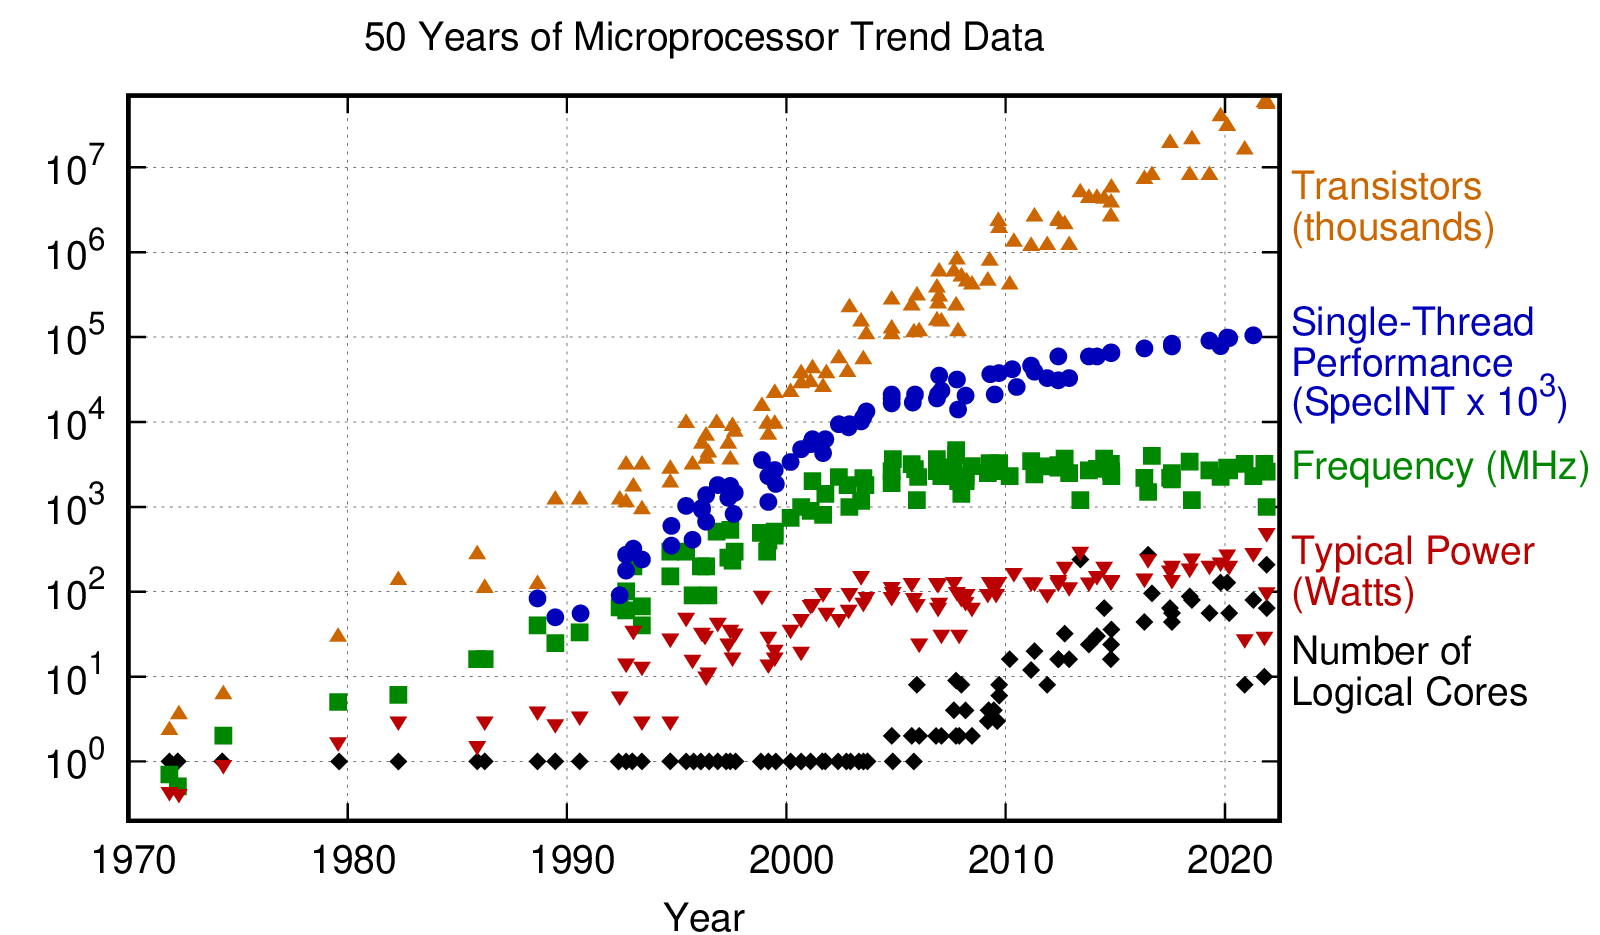
\includegraphics[width=0.8 \textwidth]{50-years-processor-trend.png}
    \caption{近50年微处理器发展趋势}
    \label{fig:processor-trend}
\end{figure}
……

\section{国内外研究现状}
本节将会对本次研究所涉及的微通道散热技术以及多热源散热技术的国内外研究进行阐述。
\subsection{微流道散热技术研究现状}
普遍学者认为,微通道指的是水力直径在 $10\ \rm{\mu m}$ 到 $1000\ \rm{\mu m}$ 范围内的通道(也有观点认为是 $1\ \rm{\mu m}$ 到 $100\ \rm{\mu m}$)所构成的换热器。
以下是较为常见的微通道尺寸分类,可以参见\cref{tab:division-of-microchannels}。
\begin{table}[htbp]
    \caption[微通道的划分]{微通道的划分\cite{LuSiHong_2021}}
    \setlength{\tabcolsep}{14mm}{ % 因表格过窄,手动设置宽度为7mm
        \begin{tabular}{lc}
            \toprule
            通道种类    & 水力直径$\mu m$   \\
            \midrule
            分子纳米通道  & $\le 0.1$     \\
            过渡性纳米通道 & $0.1\sim 1$   \\
            过渡性微通道  & $1\sim 10$    \\
            微通道     & $10\sim 1000$ \\
            常规通道    & $>1000$       \\
            \bottomrule
        \end{tabular}}
    \label{tab:division-of-microchannels}
\end{table}

在流道尺寸方面……

\subsection{多热源散热技术研究现状}
针对于单芯片散热,目前已有大量国内外学者进行相……

\subsubsection{基于基板与冷板优化分析}
在多热源散热性能的研究中多数学者集中在芯片下方的基板与冷板上进行……

\subsubsection{基于热源优化分析}
Ben Abdelmlek等人以热源的尺寸、布局和结构为切入点对多热……

\section{本文主要研究内容}
本次研究是针对应用于功率芯片的多级嵌入式散热装置的基板级散热问题所展开的研……

\noindent 本文具体研究内容如下:

\begin{enumerate}[label =(\arabic*)]

    \item 基于嵌入式散热模块的微通道流动与传热性能研究。
          将三种带有嵌入式散热模块的微通道:带有针鳍……
          最终选用MC-RPF作为核心散热结构;
    \item 分析几何参数对带有针鳍-肋嵌入式散热模块微通道流动与传热的影响。
          主要研究……;
    \item 对采用针鳍-肋嵌入式散热模块的微通道进行多目标优化。
          采用响应面分析法(Response Surface Methodology,RSM)与……;
    \item 基于MC-RPF的多热源散热结构设计分析。
          为解决在多热源应……;
    \item 基于MC-RPF的多热源散热结构压降优化。
          以压降损失相关理论为指导依据,……。

\end{enumerate}

\section{本论文的结构安排}
\cref{ch:1}:绪论。本章主要分为……。

\cref{ch:2}:相关理论基础及结构设计要求与思路。本章主要分为……。

\cref{ch:3}:基于嵌入式散热模块的微通道流动与传热性能研究。本章研究了几种……。

\cref{ch:4}:基于嵌入式散热模块的微通道多目标优化分析。本章在\cref{ch:3}完成基于……。

\cref{ch:5}:基于MC-RPF的多热源散热结构设计分析及压降优化。本章在\cref{ch:4}完成MC-RPF多目标优化……。

\cref{ch:6}:全文总结与展望。本次研究工作进行总结,并根据全文研究过程中……。


